\documentclass[titlepage,landscape]{seminar}
\usepackage{url}
\usepackage{graphicx}
\usepackage{hyperref}
\usepackage{epstopdf}
\usepackage{slides}

\newcommand{\frack}{\frac{1}{k}}
\newcommand{\quarter}{\frac{1}{4}}

\begin{document}

\myslide{
  \heading{Evolutionary biology}
  \vfil
  \begin{itemize}
    
  \item Evolutionary {\it process\/}: mutation, migration, drift, natural
    selection

    \begin{itemize}

      \item Focus typically on trying to understand the mechanics of
        what's happening or what will happen in the future.

      \item Will natural selection result in a balanced polymoprhism?

      \item Is migration sufficient to prevent divergence among
        populations?

      \end{itemize}

    \end{itemize}
  }

\myslide{
  \heading{Evolutionary biology}
  \vfil
  \begin{itemize}
    
  \item Evolutionary {\it pattern\/}: the pattern of relationships produced
    as a result of evolutionary processes

    \begin{itemize}

      \item Focus on trying to understand how the populations (or the
        sample of genes) we're studying came to have their current
        properties.

      \item How have the populations I'm studying been historically
        connected?

      \item How many substitutions have occurred between these two DNA
        sequences since they diverged?

    \end{itemize}

  \end{itemize}
}

\myslide{
  \heading{The physical basis of molecular variation}

  \begin{itemize}

\item {\bf Nucleotide sequence}: exons, introns, 5' or 3' untranslated regions),
  non-transcribed functional regions~(e.g., promoters), or regions
  without apparent function.

\item {\bf Insertion-deletion}: small (or large) segments of DNA may be
  inserted into or deleted from copies

\item {\bf Protein sequence}: not all nucleotide sequence differences lead
  to differences in protein sequences, and not all genes have DNA
  translated into protein, e.g., ribosomal RNA and various small
  nuclear RNAs.

\item {\bf Copy number variation}: 76 copy-number polymorphisms (CNPs)
  were identified in a sample of only 20 individuals, and individuals
  differed from one another by an average of 11
  CNPs.

  \end{itemize}

}

\myslide{
  \heading{Revealing molecular variation}

  \begin{itemize}

  \item {\bf isozymes}: soluble proteins separated by electrophoresis

  \item {\bf RFLPs}: restriction fragment length polymorphisms

  \item {\bf microsatellites}: short tandem repeats (2-6 nucleotides),
    differences in number of repeats

  \item {\bf nucleotide sequences}:

  \item {\bf single nucleotide polymorphisms}:

  \end{itemize}`
}


\myslide{
  \heading{Divergence of nucleotide sequences}

  How does the similarity between nucleotide sequences change over
  time?

  {\small
\begin{eqnarray*}    
  q_t &=& \mbox{probability that two nucleotide positions are identical
          after t generations} \\
  \Delta t &=& \mbox{a small interval  of time}
\end{eqnarray*}
}

{\small
\begin{eqnarray*}
q_{t+\Delta t} &=& (1 - \lambda\Delta t)^2q_t
                  + 2\left(1 - \lambda\Delta t\right)\left({1 \over
                           3}\lambda\Delta t\right)(1 - q_t)
                  + \hbox{o}(\Delta t^2) \\
               &=& (1 - 2\lambda\Delta t)q_t + \left({2 \over 3}\lambda
                                                    \Delta t\right)
                                              (1 - q_t) 
                  + \hbox{o}(\Delta t^2) \\
\end{eqnarray*}
}
}

\myslide{
\heading{Divergence of nucleotide sequences}
{\small
\begin{eqnarray*}
q_{t+\Delta t} &=& (1 - 2\lambda\Delta t)q_t + \left({2 \over 3}\lambda
                                                    \Delta t\right)
                                              (1 - q_t) 
                  + \hbox{o}(\Delta t^2) \\
q_{t+\Delta t} - q_t &=& {2 \over 3}\lambda\Delta t - {8 \over
                           3}\lambda\Delta tq_t + \hbox{o}(\Delta t^2) \\
{q_{t+\Delta t} - q_t \over \Delta t} &=& {2 \over 3}\lambda - {8 \over
3}\lambda q_t + \hbox{o}(\Delta t) \\
\lim_{\Delta t\to 0}{q_{t+\Delta t} - q_t \over \Delta t}  = {dq_t \over dt} &=& {2 \over 3}\lambda - {8
\over 3}\lambda q_t \\
q_t &=& 1 - {3 \over 4}\left(1 - e^{-8\lambda t/3}\right) \\
&& \\
d &=& 2\lambda t \\
  &=& -{3 \over 4}\ln\left[1 - {4 \over 3}(1 - q_t)\right]
\end{eqnarray*}
}
}

\myslide{
  \heading{Neutral theory of molecular evolution}

  \begin{itemize}

    \item Most allelic differences in natural populations are
      selectively neutral
      
    \item Does not mean that there are no fitness differences.

    \item Does mean that $2N_es < 1$.

  \end{itemize}
}

\myslide{
  \heading{Neutral theory of molecular evolution}
  
  The rate of molecular evolution
{\scriptsize
\begin{eqnarray*}
\mbox{\# of substitutions/generation} &=& (\mbox{\# of mutations/generation})\times(\mbox{probability
  of fixation}) \\
\lambda &=& \mu_0p_0 \\
\mu_0 &=& 2N\mu \\
p_0 &=& \frac{1}{2N} \\
\lambda &=& \mu_0p_0 \\
        &=& (2N\mu)\left(\frac{1}{2N}\right) \\
        &=& \mu 
\end{eqnarray*}
}\vfill
}

\myslide{
  \heading{Neutral theory of molecular evolution}
  
The amount of diversity at neutral loci
\begin{eqnarray*}
  f &=& \frac{1}{4N_e\mu + 1} \\
  H &=& \frac{4N_e\mu}{4N_e\mu + 1}
\end{eqnarray*}
}

\myslide{
\heading{Genetic code}
\tiny
\begin{center}
\begin{tabular}{llllllll}
\hline\hline
      & Amino &       & Amino &       & Amino &       & Amino \\
Codon & Acid  & Codon & Acid  & Codon & Acid  & Codon & Acid \\
\hline
UUU   & Phe   & UCU   & Ser   & UAU   & Tyr   & UGU   & Cys \\
UUC   & Phe   & UCC   & Ser   & UAC   & Tyr   & UGC   & Cys \\
UUA   & Leu   & UCA   & Ser   & UAA   & Stop  & UGA   & Stop \\
UUG   & Leu   & UCG   & Ser   & UAG   & Stop  & UGG   & Trp \\
      &       &       &       &       &       &       & \\
CUU   & Leu   & CCU   & Pro   & CAU   & His   & CGU   & Arg \\
CUC   & Leu   & CCC   & Pro   & CAC   & His   & CGC   & Arg \\
CUA   & Leu   & CCA   & Pro   & CAA   & Gln   & CGA   & Arg \\
CUG   & Leu   & CCG   & Pro   & CAG   & Gln   & CGG   & Arg \\
      &       &       &       &       &       &       & \\
AUU   & Ile   & ACU   & Thr   & AAU   & Asn   & AGU   & Ser \\
AUC   & Ile   & ACC   & Thr   & AAC   & Asn   & AGC   & Ser \\
AUA   & Ile   & ACA   & Thr   & AAA   & Lys   & AGA   & Arg \\
AUG   & Met   & ACG   & Thr   & AAG   & Lys   & AGG   & Arg \\
      &       &       &       &       &       &       & \\
GUU   & Val   & GCU   & Ala   & GAU   & Asp   & GGU   & Gly \\
GUC   & Val   & GCC   & Ala   & GAC   & Asp   & GGC   & Gly \\
GUA   & Val   & GCA   & Ala   & GAA   & Glu   & GGA   & Gly \\
GUG   & Val   & GCG   & Ala   & GAG   & Glu   & GGG   & Gly \\
\hline
\end{tabular}
\end{center}
}

\myslide{
\heading{Types of redundancy}
\begin{center}
\begin{tabular}{lll}
\hline\hline
      & Amino & \\
Codon & Acid  & Redundancy \\
\hline
CCU   & Pro   & 4-fold \\
CCC \\
CCA \\
CCG \\
\hline
AAU   & Asn   & 2-fold \\
AAC \\
AAA   & Lys   & 2-fold \\
AAG \\
\hline
\end{tabular}
\end{center}
}

\myslide{
\heading{Rates of synonymous and non-synonymous substitution}
\scriptsize
\begin{center}
\begin{tabular}{lcc}
\hline\hline
Locus     & Non-synonymous rate & Synonymous rate \\
\hline
Histone \\
\quad H4  & 0.00                & 3.94 \\
\quad H2  & 0.00                & 4.52 \\ 
Ribosomal proteins \\
\quad S17 & 0.06                & 2.69 \\
\quad S14 & 0.02                & 2.16 \\
Hemoglobins \& myoglobin \\
\quad $\alpha$-globin & 0.56    & 4.38 \\
\quad $\beta$-globin  & 0.78    & 2.58 \\
\quad Myoglobin       & 0.57    & 4.10 \\
Interferons \\
\quad $\gamma$  & 3.06          & 5.50 \\
\quad $\alpha$1 & 1.47          & 3.24 \\
\quad $\beta$1  & 2.38          & 5.33 \\
\hline
\end{tabular}
\end{center}
}

\myslide{
\heading{Kreitman and Aquad\'e} \\
{\small
If mutations are neutral:

\begin{itemize}

\item The substitution rate equals the mutation rate.

\item Diversity within populations will be $\frac{4N_e\mu}{4N_e\mu + 1}$

\item Therefore, the amount of divergence between two species should
  be related to the amount of diversity within each.

\end{itemize}

Example: The {\it ADH\/} locus in {\it Drosophila melanogaster\/} and
{\it D. simulans}

\begin{itemize}

\item Calculate the number of ``site equivalents'' in each region of
  the locus.

\item Calculate the number of polymorphic site equivalents

\[
\frac{25}{414+411+129} \approx 0.026
\]

\item Calculate the expected number of polymorphic sites within a
  region assuming the same fraction of polymorphic sites in each
  region. 

\end{itemize}
}
}

\myslide{
\heading{Kreitman and Aguad\'e}

{\small
\begin{center}
\begin{tabular}{l|ccc}
\hline\hline
         & 5' flanking & {\it Adh\/} locus & 3' flanking \\
\hline
Diversity$^1$ \\
\quad Observed & 9     & \color{red}{\bf 14}   & 2    \\
\quad Expected & 10.8  & 10.8 & 3.4  \\
Divergence$^2$ \\
\quad Observed & 86    & 48   & 31   \\
\quad Expected & 55    & \color{red}{\bf 76.9} & 33.1 \\
\hline
\multicolumn{4}{l}{$^1$Number of polymorphic sites within {\it
         D. melanogaster\/}} \\
\multicolumn{4}{l}{$^2$Number of nucleotide differences between {\it
         D. melanogaster\/} and {\it D. simulans}}
\end{tabular}
\end{center}
}

}

\myslide{
\heading{Kreitman and Hudson}

\begin{center}
\resizebox{\textwidth}{!}{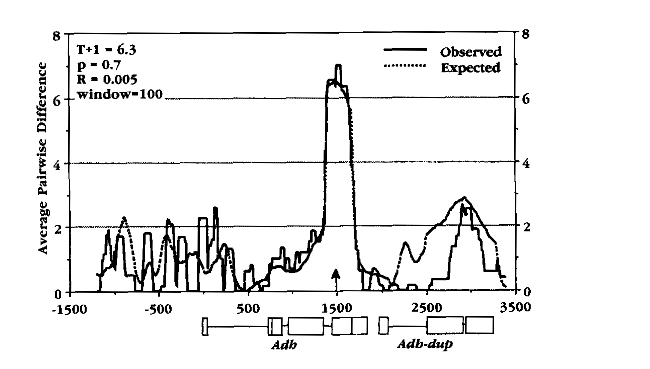
\includegraphics{kreitman-hudson.eps}}
\end{center}

}

\myslide{
\heading{$F_{ST}$ outliers}

\begin{center}
\resizebox{\textwidth}{!}{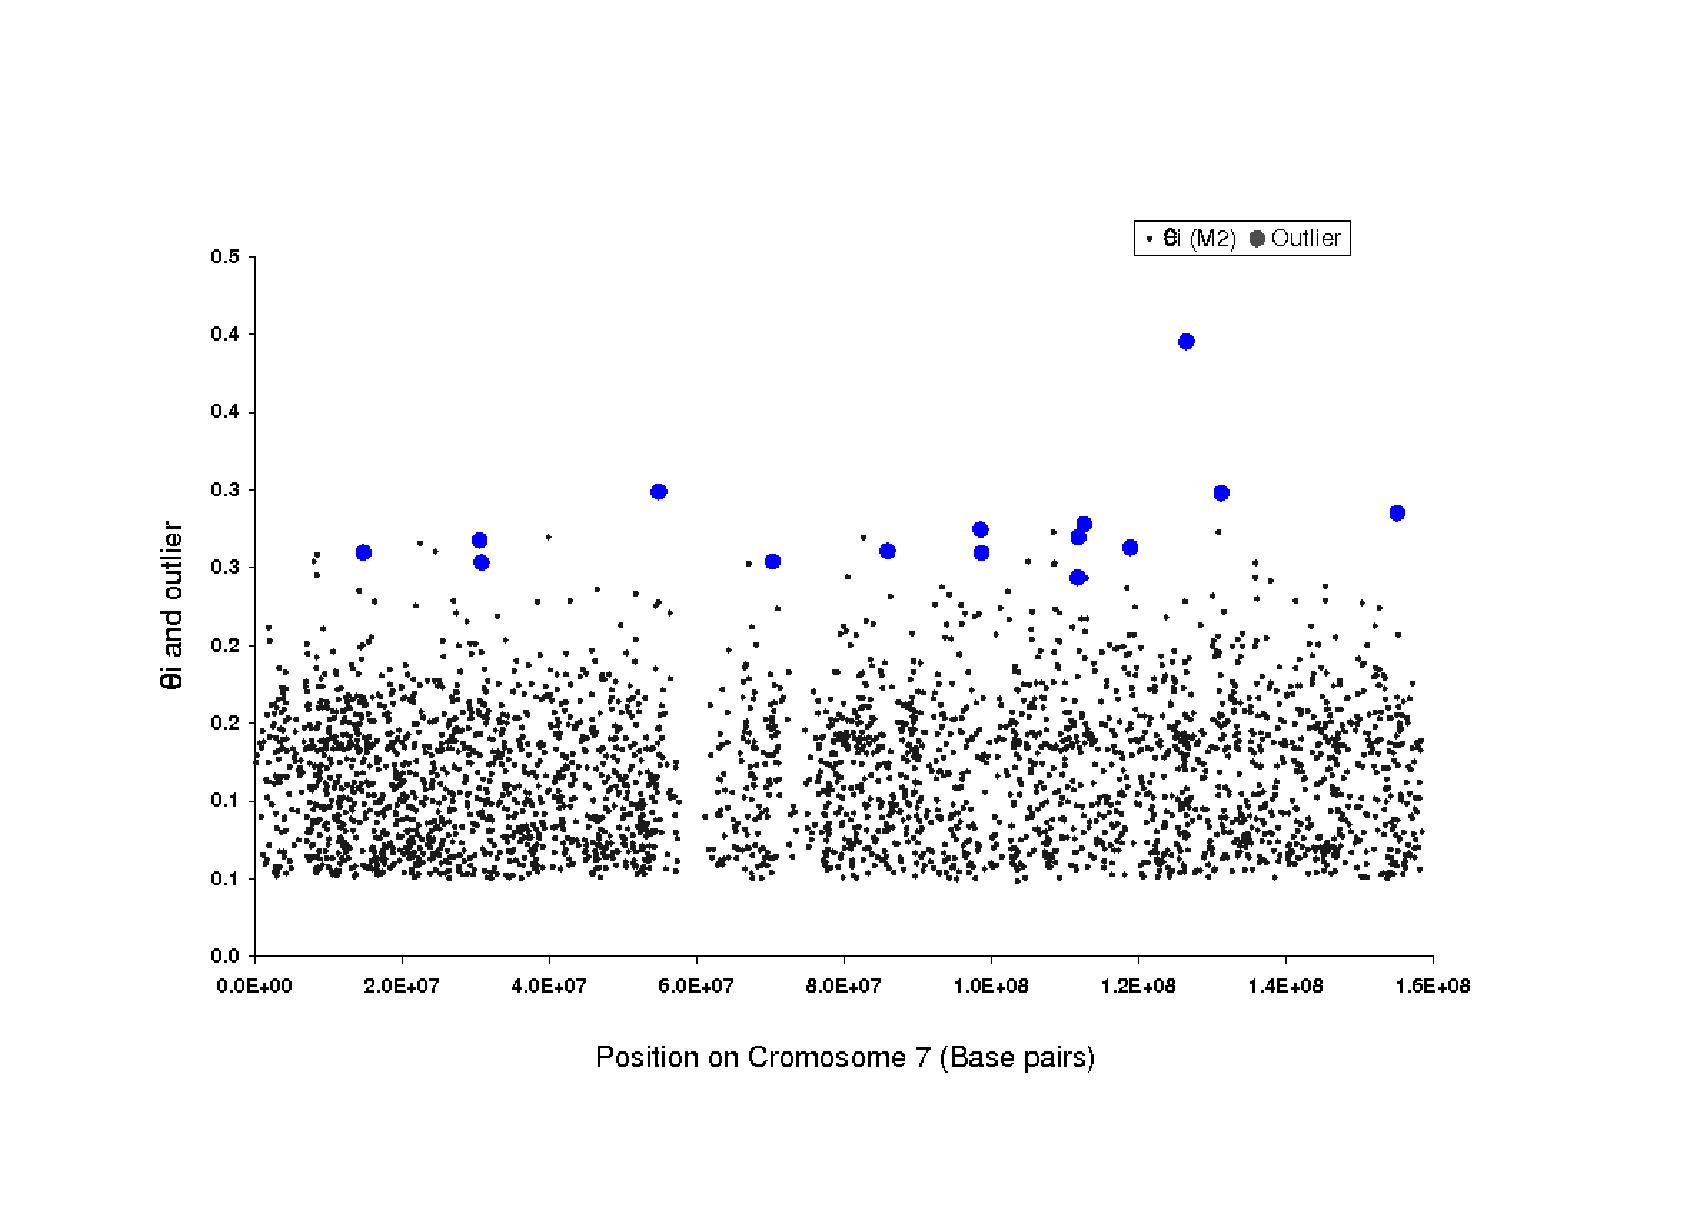
\includegraphics{outlier.eps}}
\end{center}

}

\myslide{
\heading{$F_{ST}$ outliers}

\begin{center}
\resizebox{0.9\textwidth}{!}{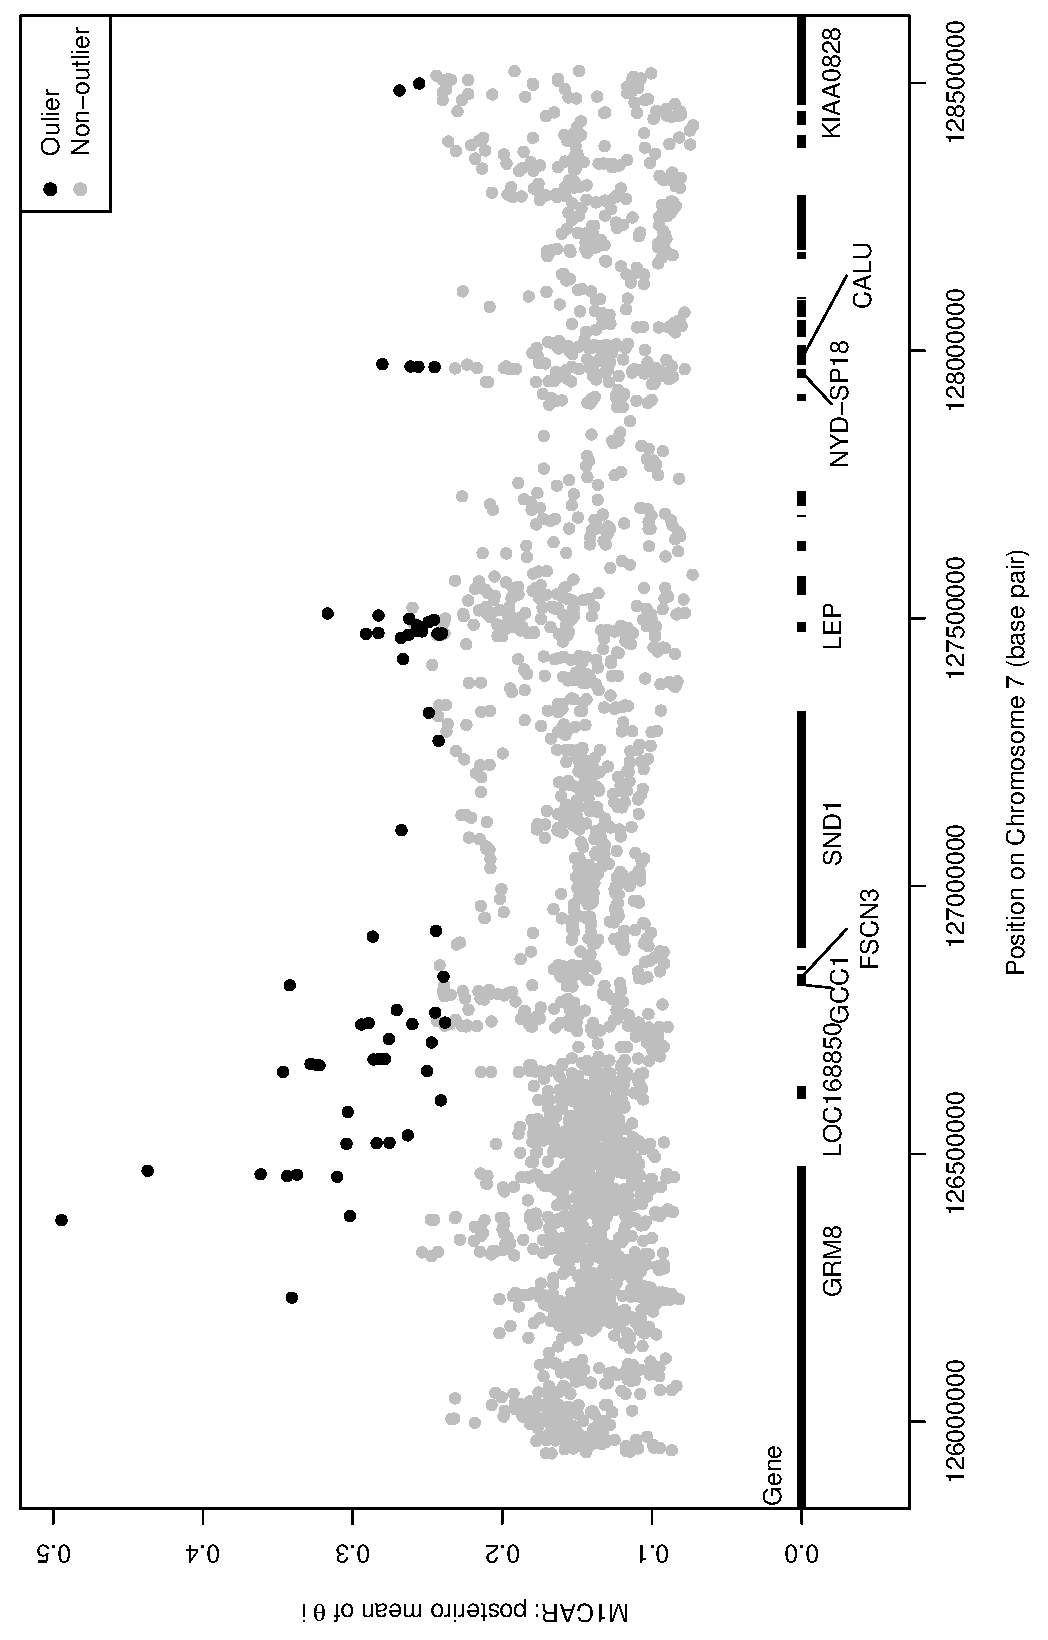
\includegraphics[angle=270]{outlier-high.eps}}
\end{center}

}

\myslide{
\heading{Segregating sites and nucleotide diversity}

\begin{eqnarray*}
k &=& \mbox{number of segregating sites} \\
\hat \pi &=& \sum x_ix_j\delta_{ij}/N ,
\end{eqnarray*}
where $x_i$ is the frequency of haplotype $i$, $\delta_{ij}$ is the
number of nucleotide differences between $i$ and $j$, and $N$ is the
sequence length.
}

\myslide{
\heading{Tajima's $D$}

Let $\theta = 4N_e\mu$. {\bf NOTE}: This is not the same $\theta$ we
encountered when we were doing $F$-statistics.

\begin{eqnarray*}
\mbox{E}(k) &=& \theta \sum_i^{n-1} \frac{1}{i} \\
\mbox{E}(\pi) &=& \theta
\end{eqnarray*}

Two estimates of $\theta$:

\begin{eqnarray*}
\hat\theta_{\pi} &=& \hat \pi \\
\hat\theta_k &=& \frac{k}{\sum_i^{n-1} \frac{1}{i}}
\end{eqnarray*}
}

\myslide{
\heading{Tajima's $D$}

\[
\hat D = \theta_{\pi} - \theta_k
\]

\begin{description}

\item[Neutral variation] $\hat D \approx 0$ 

\item[Overdominant selection] $\hat D > 0$

\item[Population bottleneck] $\hat D > 0$

\item[Purifying selection] $\hat D < 0$

\item[Population expansion] $\hat D < 0$

\end{description}

}

\end{document}

